\documentclass[10pt]{article}
\usepackage{hyperref}
\usepackage{graphicx}
\usepackage{geometry}
\geometry{legalpaper, portrait, margin=0.5in}
\oddsidemargin -0.5in
\evensidemargin -0.5in
\textwidth=6.0in
\itemsep=0in
%\parsep=0in
\topmargin=-60pt
\topskip=0in
\marginparwidth=10pt
\marginparsep=0pt
\footskip=250pt
\hoffset=0pt
\voffset=-10pt

\begin{document}
\huge{\textbf{\hspace{1.7in}Gorantla Balaji}} \\
||||||||||||||||||||||||||||||
\centering 
\thispagestyle{empty}
\large{\vspace{.05in}
\begin{tabular}{@{}p{3.5in}p{3in}}
\#1395            & \hspace{1.0cm} {Contact:}  9731302831 \\
Carstreet
 & \hspace{1cm}
  {E-mail:}\hspace{1.4mm}balajigorantla96@gmail.com\\
Kurugodu\\
PIN:583116 & {}\\
Ballari dist\\
Karnataka


\end{tabular}
}

 \begin{figure}[h]
\hspace{4.2in}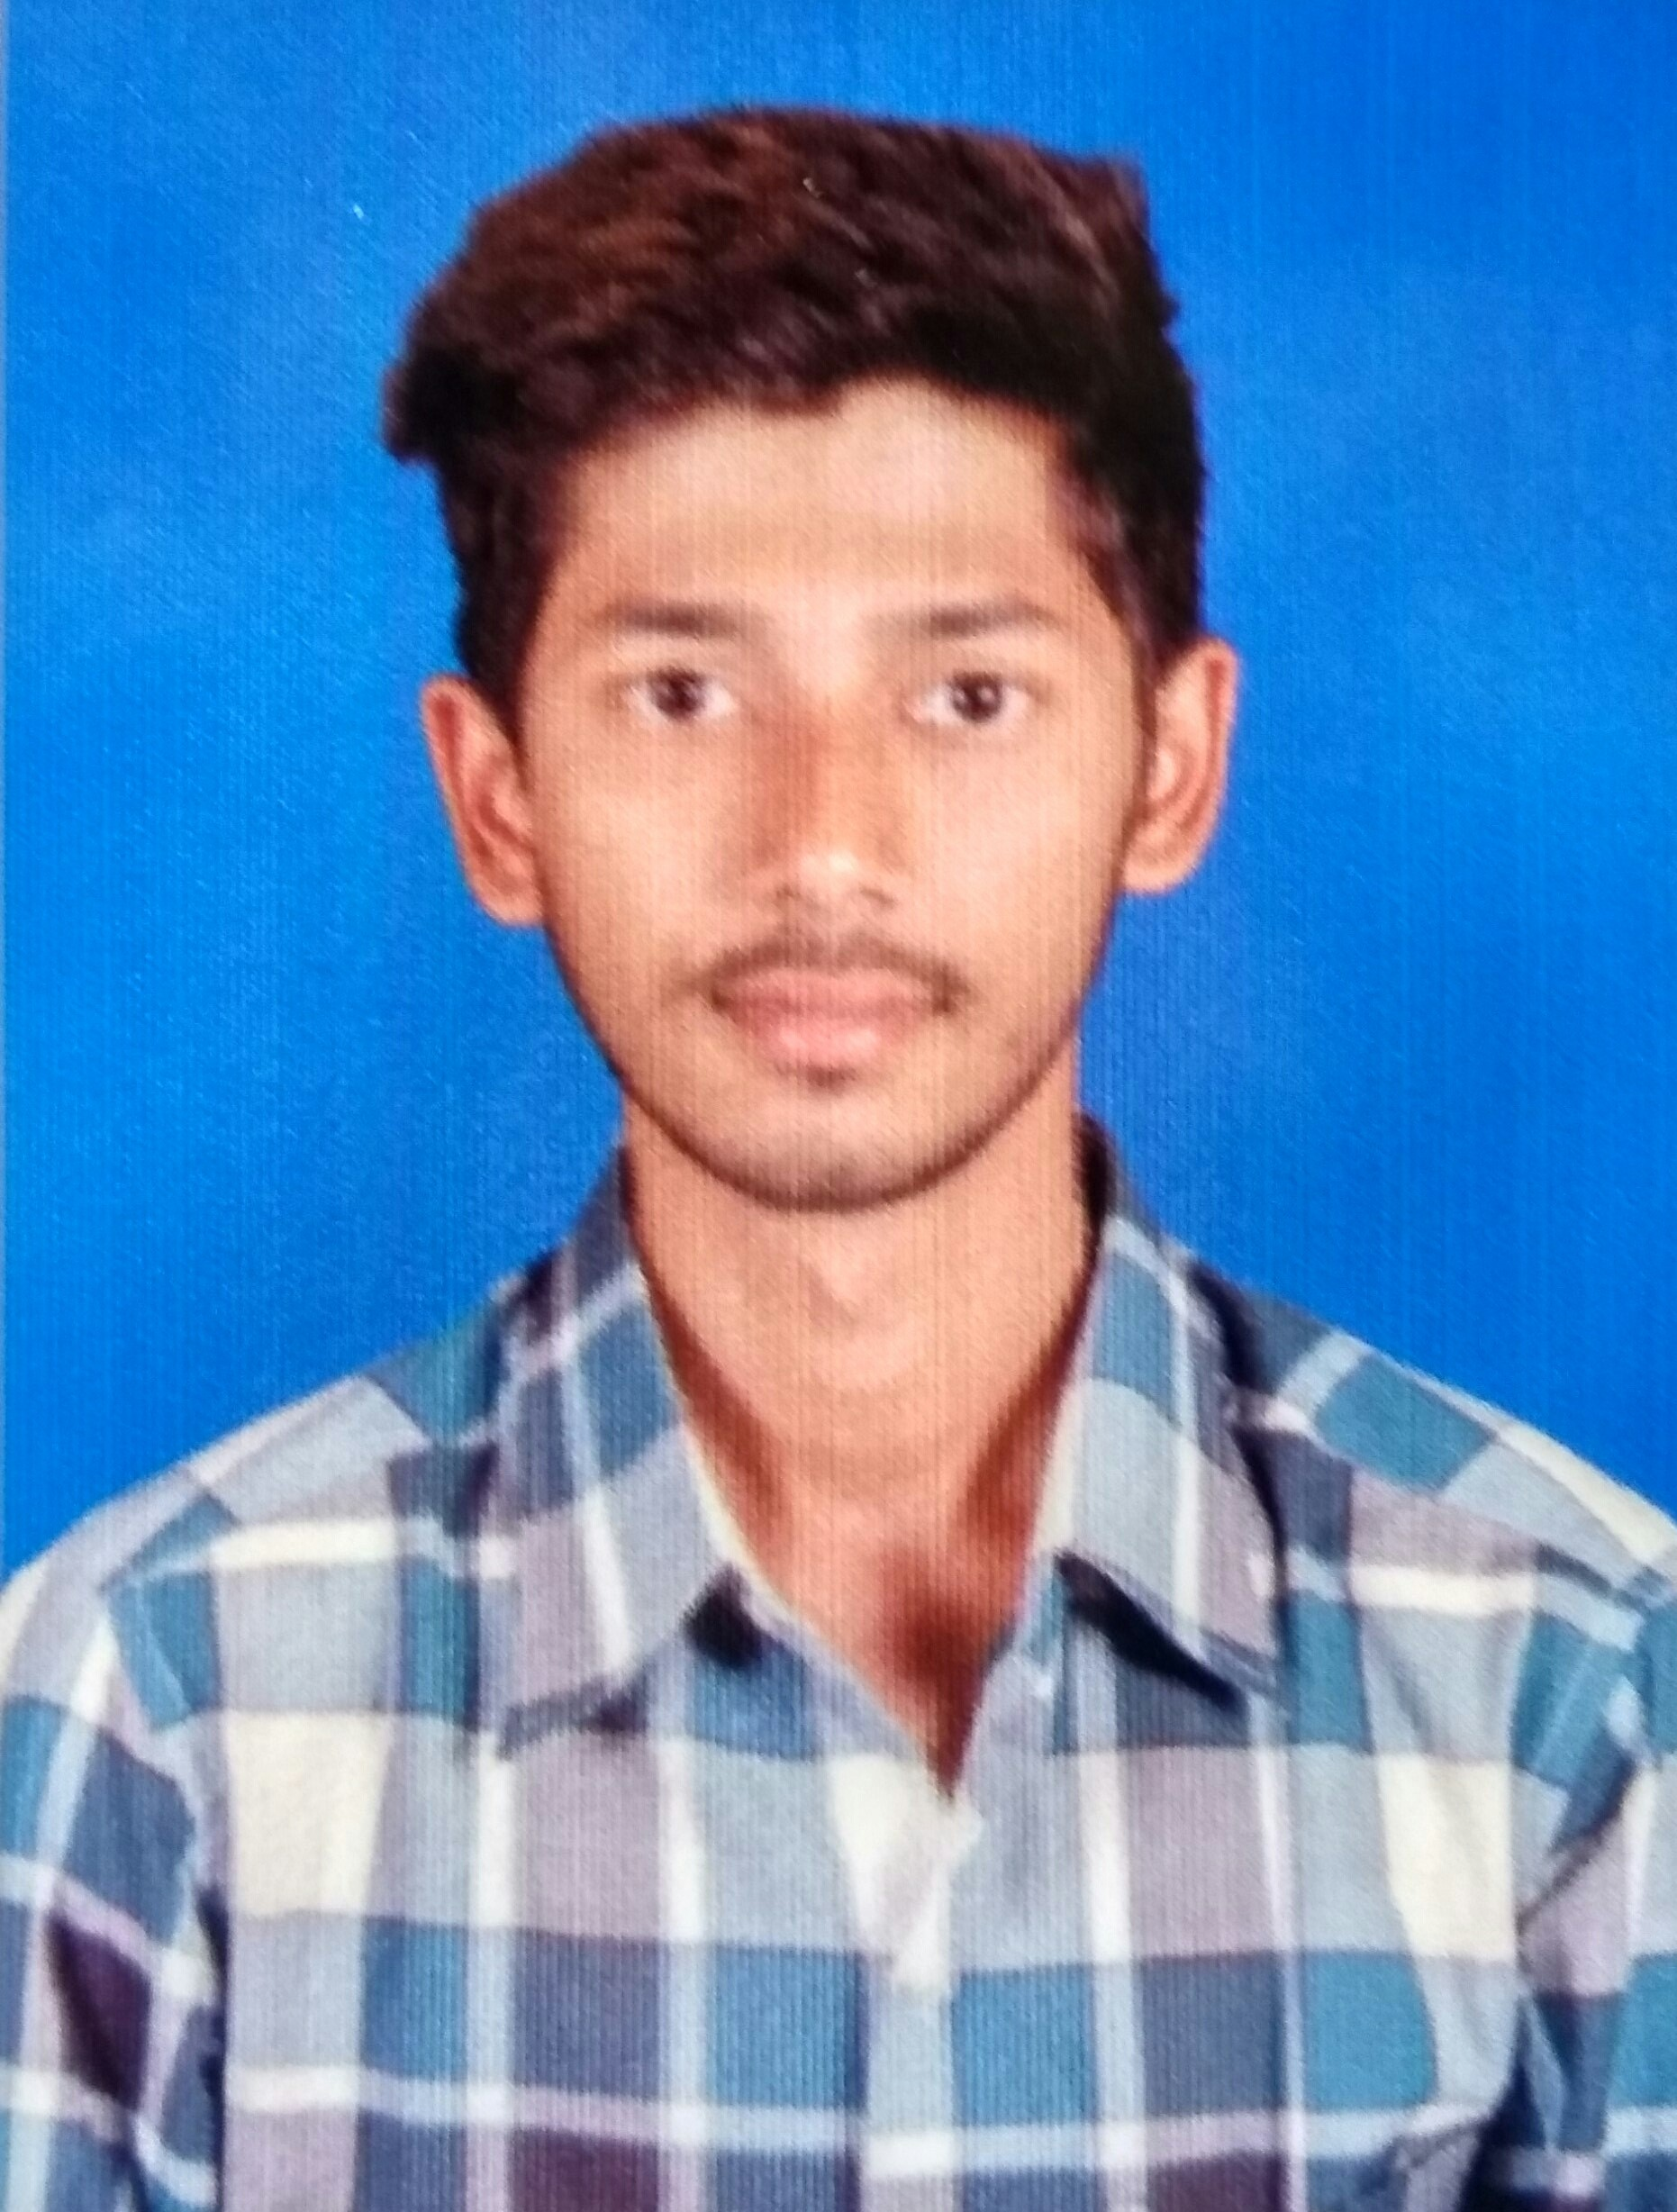
\includegraphics[scale=0.06]{IMG_20170423_160215.jpg}
\end{figure}


\raggedright
\section*{\large{OBJECTIVE}}
\hspace{2in} \large{I want to succeed in a stimulating and challenging \\\hspace{2.05in}environment, with hard work, perseverance and \\\hspace{2.05in}dedication from which I can serve my nation. }

\raggedright
\section*{\large{EDUCATION}}
\hspace{2in} \small\begin{tabular}{|c|c|c|c|c|}
\hline
\textbf{Degree} & \textbf{College/School} & \textbf{University} & \textbf{Passing Year} & \textbf{Pass Percentage/CGPA} \\
\hline
X & Vidya Residential School & KBSE & 2012 & 92.64\%\\
\hline
XII & Nandi PU College & KBPUE & 2014 & 93.16\% \\
\hline
B.E. & BMSCE  & VTU & 2018 & 8.9 \\
\hline
\end{tabular}

\raggedright
\section*{\large{PROJECTS}}
\hspace{2in} \large{1.KK 2.0 RC Quadcopter} \\
\hspace{2.5in} \large{Built a quadcopter with KK 2.0 control board\\\hspace{2.5in} with stable control sysytem.} \\
\hspace{2in} 2.DTMF technology based robot \\
\hspace{2.5in} \large{Built a robot with DTMF technology. We can\\\hspace{2.5in} control the bot with our mobile keypad from\\\hspace{2.5in} any distance. } \\
\hspace{2in} 3. RC Planes  \\
\hspace{2.5in} \large{Built 5 RC planes of different designs with wing \\\hspace{2.58in}span of around 1m  for the SAE International\\\hspace{2.5in} Aero Design competetions and for general \\\hspace{2.58in}projects. } \\
 

\raggedright
\section*{\large{TRAINING \& \hspace{8in} INTERNSHIPS}}
\hspace{2in} \large{Attended numorous workshops on -  }\\
\hspace{2.5in} \large{1.Quadcopter designing.}\\
\hspace{2.5in} \large{2.AVR programming.}\\

\raggedright
\section*{\large{RESEARCH \hspace{8in} PUBLICATIONS}}
\hspace{2in} None as of yet.\\

\raggedright
\section*{\large{TECHNICAL \hspace{8in} SKILLS}}
\hspace{2in} \large{1. Programming languages }\\
\hspace{2.5in} \large{C, C++, Assembly.  }\\
\hspace{2in} \large{2.Aerospace }\\
\hspace{2.5in} \large{ Avionics, Aero designing. }\\
\hspace{2in} \large{3.softwares }\\
\hspace{2.5in} \large{MATLAB,Cadence, Photoshop, Illustrator,\\ \hspace{2.5in} LaTeX, Proteus, LTSpice, Keil, Xilinx Vivado,\\\hspace{2.5in}  Sketchup.}\\

\raggedright
\section*{\large{SOFT \hspace{8in} SKILLS}}
\hspace{2in} \large{ Leadership, Self-Motivation, Team Player,\\ \hspace{2.05in} Responsible, Problem Solving, Ability to Work Under\\ \hspace{2.05in} Pressure and Time Management, Flexible,\\\hspace{2.05in} Decisiveness.}\\

\raggedright
\section*{\large{EXTRA- \hspace{8in}CURRICULAR \hspace{8in}ACTIVITIES}}
\hspace{2in} \large{ 1. Fine Arts- }\\
\hspace{2.5in} \large{ -winner in Chintana state level sketching\\ \hspace{2.65in}  competetion. }\\
\hspace{2.5in} \large{ -winner in inter-college best out of waste\\ \hspace{2.65in} creative competetion.}\\
\hspace{2in} \large{ 2.Sports-  }\\
\hspace{2.5in} \large{ -runner in District level Chess. }\\
\hspace{2.5in} \large{ -winner in Taluk level shuttle badminton. }\\
\hspace{2.5in} \large{ -winnner in Intra-College Kho-Kho\\ \hspace{2.65in}competetion. }\\
\hspace{2in} \large{ 3.Culturals }\\
\hspace{2.5in} \large{ -Dance.}\\
\hspace{2.5in} \large{ -Theatre.}\\

\raggedright
\section*{\large{CO- \hspace{8in}CURRICULAR \hspace{8in}ACTIVITIES}}
\hspace{2in} \large{ 1. Coordinated NSS Unit, BMSCE for the academic\\ \hspace{2.3in} year 2016-17.}\\
\hspace{2in} \large{ 2. Coordinated Aerospace Club, BMSCE for the \\ \hspace{2.3in}academic year 2016-17. }\\
\hspace{2in} \large{ 3. Conducted workshops on RC plane design \\ \hspace{2.3in}fabrications. }\\

\section*{\large{PERSONAL \hspace{8in}DETAILS}}
\large{\vspace{.05in}
\begin{tabular}{@{}p{3.5in}p{3in}}
\hspace{2in}Father's name: &  G Suresh \\
\hspace{2in}Mother's name: &  G Vijaya Lakshmi\\
\hspace{2in}Sex: & Male\\
\hspace{2in}Date of Birth:  & 21/07/2017\\
\hspace{2in}Nationality: & Indian\\
\hspace{2in}Marital Status: & Single

\end{tabular}

\section*{\large{REFERENCE}}
\hspace{2in} S Lalita (Student Proctor) \\
\hspace{2in} Contact: 9886252648.

\section*{\large{DECLARATION}}
\hspace{2in}  I hereby declare that the above cited information is\\\hspace{2in} true to the best of my knowledge and belief, if given a\\\hspace{2in} chance, I can prove myself.
\section*{\large{DATE}}
\hspace{2in} 24-04-2017

\end{document}